% !TEX root = ../Documentation.tex

\section{Design}
\label{sec:design}

\subsection{System overview (D)}
  The parser module overview is given in \autoref{fig:ParserModules}.
  Each of the modules are described in the following subsection.
  %
  \begin{figure}[ht]%
    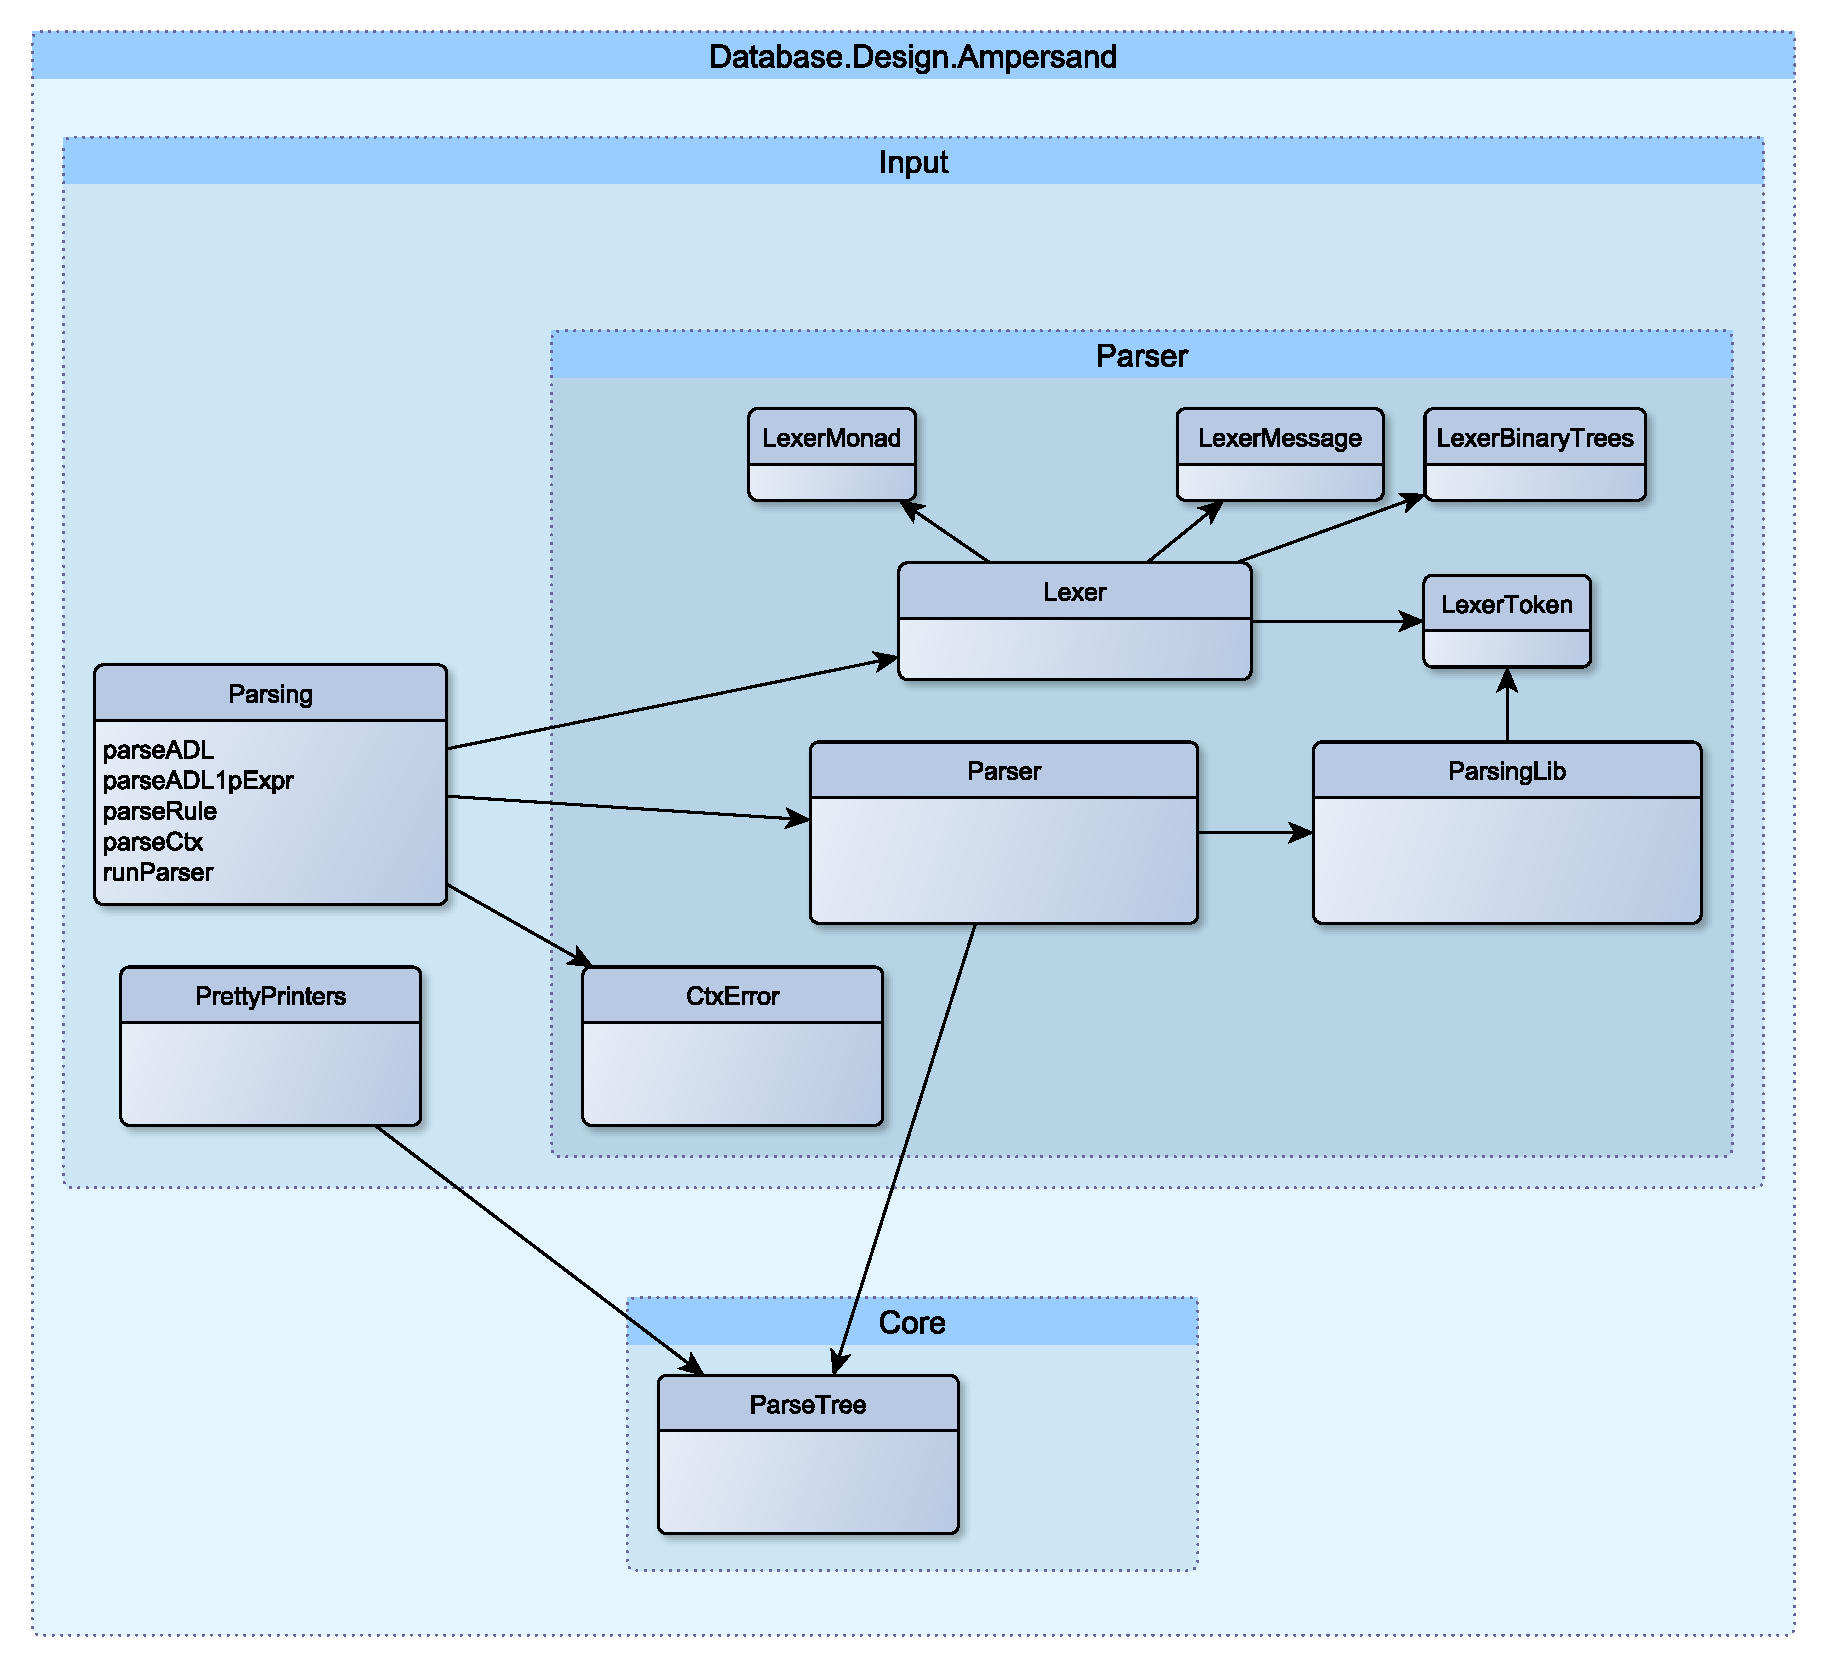
\includegraphics[width=\columnwidth]{Figures/ParserModules}
    \caption{The parser modules and their relationships}
    \label{fig:ParserModules}
  \end{figure}%
  TODO: Add the exported functions to each module.

  \subsubsection{Modules}
  \label{subsec:parser-modules}
  In this section a short description of each module is given:
  %
  \begin{description}
    \item[Parsing] module that implements the interface of the parser with the rest of the system.
      It is responsible for reading the input files, calling the lexer and the parser and returning a parse tree as result (or a parse error).

    \item[Parser] module responsible for executing the parsing itself.
      It accepts the tokens that are allowed in each grammar production and generates the corresponding parse tree.
      The parser is described in \autoref{subsec:design-parser}.
      
    \item[ParsingLib] library that contains several useful functions to assist the parser, e.g. token recognition.
      These functions are not depending on the specific grammar rules.
      
    \item[ParseTree] external module containing the parse tree data structures.
      Only details of this module have been changed during this project (e.g. field ordering).
    
    \item[PrettyPrinters] contains the \texttt{Pretty} class and the functions responsible for printing the parse tree to ADL scripts in a `pretty' way.
    
    \item[CtxError] contains the data structures responsible for the parse errors and their location.
      This module has not been refactored as a part of this project.
    
    \item[Lexer] module responsible for recognizing the input characters and converting them to tokens.
      The lexer is described in \autoref{subsec:lexer}.
    
    \item[LexerMonad] contains a monad definition that supports lexing with context.
      It tracks for example the location in the input and the warnings that may be generated.
    
    \item[LexerMessage] contains functions to handle errors and warnings from the lexer.
    
    \item[LexerBinaryTrees] module responsible for searching binary trees in an efficient way, to support the token recognition.
    
    \item[LexerToken] contains the data structure that represents the input tokens for the lexer.
      The tokens work as an interface between the lexer and the parsing library.
  \end{description}

\subsection{Changes due to Parsec (D)}
TODO: Show the differences between uulib and Parsec, e.g. the try for backtracking.

\subsection{Lexer (M)}
\label{subsec:lexer}
TODO: describe how the lexer works, and the improvements done to it.

\subsection{Parser (D)}
\label{subsec:design-parser}
The mainstream design of the new parser has not changed much.
Basically, each EBNF rule receives its own parser function.
Thanks to the combinator operators, the parsing function also looks very similar to the EBNF.

The applicative interface is consistently used.
By changing details of the implementation, e.g. the order of the fields in the parse tree, we have made many of the `rebuild' functions unnecessary.
For some parsers the amount of changes necessary in order to use a purely applicative style was too large or even impossible with the current parse tree.

\subsubsection{Parsec (D)}
\label{subsec:design-parsing-lib}
As mentioned earlier, and described in research context document \citenac{parsing}, the new Ampersand parser has been rebuilt with another parsing library, namely Parsec.
However, for the Ampersand developers, the source code of the parser will still look very familiar, thanks to the applicative interface.
For developers, the main differences between Parsec and the uulib are:
\begin{itemize}
  \item Parsec does not backtrack by default.
    In order to enable backtracking, the `try' function must be used.
    This is described in \autoref{subsec:backtracking}.
  \item Parsec does not try to solve parsing errors.
    The parser stops immediately after the first issue.
    Se also the error analysis in \autoref{subsec:design-errors}.
  \item Error messages are customizable by using the <?> operator.
    This is also suggested in \autoref{subsec:design-next-steps}.
\end{itemize}

\subsubsection{Backtracking (D)}
\label{subsec:backtracking}
In order to explain the differences on backtracking behavior between the uulib and Parsec, we quote Doaitse Swierstra here:
\begin{quote}
\textsl{To understand the subtleties it is important to understand the differences between the try construct in Haskell and the non-greedy parsing strategy used in uu-parsinglib. Effectively the latter is a try which just looks ahead one symbol. In that respect it is less powerful than the try construct from Parsec, in which you specify that a specific construct has to be present completely. And then there is the underlying different overall strategy. Parsec uses a back-tracking strategy with explicit tries to commit, whereas uu-parsinglib uses a breadth-first strategy with an occasional single symbol look-ahead.}
\end{quote}
%
We can therefore conclude that the try-statements in Parsec are undesirable.
However, they are necessary when the grammar is ambiguous.
In this section we explain why each of the remaining try statements are necessary, and how the issues with the grammar can be resolved:
\begin{description}
  \item[Classify]
    pClassify vs pGenDef
  
  \item[Role]
    pRoleRelation vs pRoleRule
  
  \item[Population]
    pPopulation with pNamedRel or pConceptName
  
  \item[View]
    pFancyViewDef vs pViewDefLegacy
  
  \item[Content]
    pContent
  
  \item[Multiplicity]
    pFun.pMult
  
  \item[Labels and Terms]
    opLabelProps + pTerm in pIndex and pViewAtt, pLabel + pRule in pRuleDef
\end{description}

\subsection{Parse tree (R-M)}
\label{subsec:design-parse-tree}
Improvements in the Ampersand parse tree are out of the scope of this project, because of the potential consequences to the rest of the Ampersand system.
However, during the development of the new parser a few constructions have been changed in order to make the parser more readable and maintainable.
The changes have been mostly in the order of the constructor parameters, and this was done consequently though all Ampersand modules.
The updated parse tree is depicted in the appendices (\autoref{fig:parse-tree}).

\subsection{Errors (M)}
\label{subsec:design-errors}
TODO: show what we've done to improve the errors.

\subsection{Next steps (M)}
\label{subsec:design-next-steps}
TODO: give tips on how to further improve the parser. e.g.:
  - cleanup CtxError, add warnings, use <?> for the errors.
  - reorganize parse tree, e.g. using always Origin as first parameter.